%=====================================================================
\section{Experimental setup}\label{sec:setup}
%=====================================================================

\subsection{Data}\label{sec:data}
We use four public 12-lead databases from three countries (Table~\ref{tab:datasets}, Fig.~\ref{fig:demo}): the China Physiological Signal Challenge 2018 database together with its extra set (CPSC2018 and CPSC-Extra, pooled as ``CPSC'')~\cite{liu_cpsc2018,perez2020}, PTB-XL from Germany~\cite{wagner2020}, the Georgia 12-lead ECG Challenge database from the United States~\cite{perez2020}, and the Shaoxing and Ningbo First Hospital database from China~\cite{zheng2020,zheng2022ningbo}, as redistributed by the PhysioNet/CinC 2021 Challenge~\cite{reyna2022} and hosted on PhysioNet~\cite{goldberger2000}. The two further Challenge sources, the St.~Petersburg INCART database (long Holter recordings) and the original PTB database, are too small to serve as held-out targets and are excluded. CPSC comprises two releases of one challenge and Shaoxing--Ningbo pools two hospitals released together; we therefore speak of databases rather than hospitals. Diagnoses are SNOMED-CT codes from the record headers; the four code equivalences defined by the 2021 Challenge are applied to all methods before anything else (Table~\ref{tab:rules}). Records shorter than 5\,s, flat records and duplicates are discarded during preprocessing, which removes two recordings and leaves 87{,}661 recordings in the four databases. All recordings were acquired at 500\,Hz; PTB-XL, Georgia and Shaoxing--Ningbo recordings last at most 10\,s, whereas CPSC recordings last 6--144\,s (median 12\,s).

The global vocabulary $\mathcal{V}$ consists of the diagnoses for which a clinical description was written (Supplementary Table~S1) and which have at least 50 positive recordings across the four databases and at least ten in one of them; it contains $C=43$ diagnoses, of which 25 belong to the 26 classes scored in the 2021 Challenge and the remainder are frequent unscored codes. A database \emph{annotates} a diagnosis when it has at least ten positive recordings of it. Table~\ref{tab:datasets} reports the size of each annotated vocabulary, Fig.~\ref{fig:annot} shows the full coverage pattern, and Supplementary Table~S2 gives the full database-by-diagnosis count matrix. All counts are computed from the output of the preprocessing script and are not edited by hand.

\begin{table}[t]\centering\footnotesize\setlength{\tabcolsep}{4pt}
\caption{Databases used in this study after excluding recordings shorter than 5\,s, flat recordings and duplicates (two recordings in total). All recordings were sampled at 500\,Hz. Duration in seconds, median (range). Age excludes missing values and the PTB-XL anonymization code (300) used for patients older than 89 years. Annotated = number of vocabulary diagnoses with at least ten positive recordings in the database.}\label{tab:datasets}
\begin{tabular*}{\textwidth}{@{\extracolsep{\fill}}llrcccr@{}}\toprule
Database & Country & Records & Duration (s) & Age (years) & Female (\%) & Annotated \\ \midrule
CPSC & China & 10,328 & 12 (6--144) & 61.4 $\pm$ 18.0 & 46.3 & 24 \\
PTB-XL & Germany & 21,837 & 10 (10--10) & 59.5 $\pm$ 16.8 & 47.9 & 32 \\
Georgia & USA & 10,344 & 10 (5--10) & 60.5 $\pm$ 15.4 & 46.3 & 33 \\
Shaoxing--Ningbo & China & 45,152 & 10 (10--10) & 58.2 $\pm$ 19.7 & 43.6 & 41 \\
\midrule Total & & 87,661 & & & & 43 \\
\bottomrule\end{tabular*}\end{table}


\begin{figure}[!htbp]
\centering
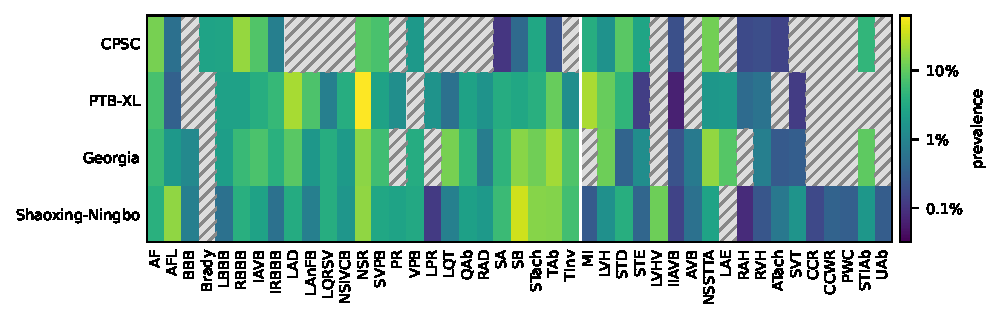
\includegraphics[width=\textwidth]{figures/fig_annotation_matrix.pdf}
\caption{Annotation coverage of the four databases over the $C=43$ vocabulary diagnoses. Colour gives the prevalence of each diagnosis in each database on a logarithmic scale; hatched cells mark diagnoses that the database does not annotate (fewer than ten positive recordings). Only 18 of the 43 diagnoses are annotated by all four databases, and 16.7\% of all record--diagnosis entries in the pooled label matrix are unknown rather than negative. Under naive pooling every hatched cell is treated as a confirmed negative.}\label{fig:annot}
\end{figure}

\begin{figure}[!htbp]
\centering
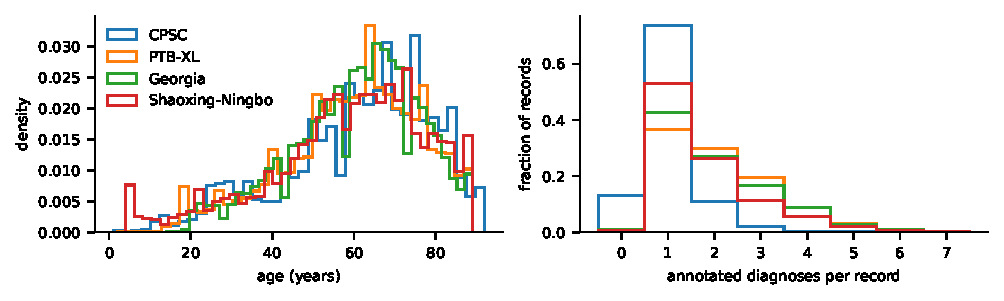
\includegraphics[width=\textwidth]{figures/fig_demographics.pdf}
\caption{Population characteristics of the four databases. Ages above 89 years are coded as 300 in PTB-XL for anonymity and are excluded from the age statistics.}\label{fig:demo}
\end{figure}


\subsection{Protocols}\label{sec:protocols}
\paragraph{E1: leave-one-database-out.}
Each of the four databases is held out in turn. The model is trained on the pooled records of the other three, of which a fixed random 10\% (split seed 0) serves as the validation split for model selection and threshold tuning, and tested on all records of the held-out database, restricted to the diagnoses that database annotates. Diagnoses annotated by at least one training source are reported as \emph{seen}; those annotated only by the held-out database are \emph{unseen}. The partition and the indicator $\kappa_c$ are computed from the raw annotation rule before implication completion, so it is a property of the fold, not of the method. Two folds have evaluable unseen diagnoses: CPSC (bradycardia, one diagnosis) and Shaoxing--Ningbo (left ventricular high voltage, clockwise and counterclockwise cardiac rotation, P-wave change and abnormal U wave; five diagnoses). Bradycardia is the implied finding of the rule sinus bradycardia $\rightarrow$ bradycardia, so every method that uses implication completion receives positive-only supervision for it when CPSC is held out; the five Shaoxing--Ningbo diagnoses receive no supervision of any kind. Unseen diagnoses can be scored meaningfully only by models without diagnosis-specific weights; we nevertheless report the linear-head baselines on them, whose untrained rows provide an empirical chance reference.

\paragraph{E2: controlled annotation removal.}
To isolate the effect of the objective from that of the data, we simulate heterogeneous annotation on a single database. PTB-XL records are split at random into 80\% training, 10\% validation and 10\% test (patient identifiers are not included in the Challenge redistribution, so the split is by record). Each diagnosis that PTB-XL annotates is then removed from the training supervision independently with probability $r\in\{0,0.25,0.5\}$ (sinus rhythm is protected), as if PTB-XL had never coded it: the corresponding targets become zero and the corresponding entries become unobserved. The removed diagnoses are drawn once per rate with a fixed seed, from the raw annotation and before implication completion, and are shared by all methods; at $r=0.25$ seven diagnoses are removed and at $r=0.5$ seventeen (listed in Supplementary Table~S4). Naive pooling, the Li-style baseline and the proposed method are trained on the altered supervision and evaluated against the complete original labels, separately over the retained and the removed diagnoses. A removed diagnosis is annotated by no training record, so for the proposed method it is an unseen diagnosis scored by the text head, while for the baselines its linear row receives only negative targets (naive) or no gradient at all (Li-style), unless an implication rule completes it. Because a single source offers no source shortcut, E2 isolates the effect of label handling from that of distribution shift.

\paragraph{E3: systematic zero-shot evaluation.}
E1 contains only six genuinely unseen diagnoses, in two folds. To evaluate open-vocabulary scoring on a broad and pre-specified set of diagnoses, E3 withholds diagnoses that would normally be seen. In each leave-one-database-out fold, every diagnosis that the held-out database annotates and that at least one training source annotates (sinus rhythm excepted) is assigned to one of 4--6 fixed groups of about six diagnoses, drawn at random once (seed 0) and listed in Supplementary Table~S5. Each run withholds one group: its columns are removed from the raw labels \emph{before} implication completion, so that no trained diagnosis is completed from a withheld one, and they never enter the loss. The withheld diagnoses are then scored on the held-out database by the text head alone. Every eligible diagnosis is thus scored zero-shot exactly once per fold and seed, giving 120 (database, diagnosis) pairs over four folds, each with three seeds (60 training runs). For each pair we compare the zero-shot AUROC with chance, with the AUROC that the same model obtains when the diagnosis is trained (from E1), and with the zero-shot AUROC of a report-pretrained ECG--language model (Section~\ref{sec:baselines}). We also test whether zero-shot accuracy depends on the cosine similarity between the description anchor of the withheld diagnosis and the nearest anchor of a trained diagnosis.

\paragraph{Annotation threshold and calibration.}
The proposed method and the Li-style baseline are re-run on all folds (seed 0) with the annotation threshold set to 5 and to 20 positives instead of 10; both the vocabulary and the annotated sets change accordingly. Calibration on seen diagnoses is assessed for all methods from the E1 test predictions by the expected calibration error (15 equal-width bins), the Brier score and the ratio of mean predicted probability to observed prevalence; no method is recalibrated.

\paragraph{Ablations.}
Four variants of the proposed method, run under E1 with three seeds, change one design decision each: (i) \emph{linear scoring} scores seen diagnoses by the linear head alone, so the text head acts only as an auxiliary training task on the shared encoder and as the scorer of unseen diagnoses; (ii) \emph{detached text head} stops the gradient of the text-head loss into the encoder, so that the encoder is trained exactly as in the Li-style baseline and the hybrid reduces to a post-hoc ensemble of two heads; (iii) \emph{+ pseudo-labels} adds soft pseudo-labels from the averaged model on unobserved entries of seen diagnoses, applied to the text head from the third epoch; and (iv) \emph{text head only} is the strongest single-head text-anchored model from our development sweep, in which a class-specific residual (bias, query read-out and pooled read-out for seen diagnoses) is added to the text logit and soft pseudo-labels with soft implication consistency are used (Appendix~\ref{secA2}). A second group of seven single-seed ablations of an earlier text-only model (learned instead of text queries, name-only descriptions, a general-domain text encoder, removal of implication completion, of MixStyle or of the text head) is reported in Appendix~\ref{secA2}.

\subsection{Baselines}\label{sec:baselines}
All baselines share the encoder, preprocessing, augmentation including lead dropout, loss function, optimizer, schedule, weight averaging and model-selection rule of the proposed method; they differ only in how labels and sources are handled, and all use the linear head of Eq.~\eqref{eq:linear}. \textbf{Naive pooling} treats every unannotated entry as a negative. \textbf{Masked} ignores unannotated entries (Eq.~\eqref{eq:lann}). \textbf{Li-style} combines masking with implication-based completion of the targets, following the prediction-masking and category-mapping idea of Li et al.~\cite{li2024}; it is a re-implementation of that label handling within our shared training framework, not their original code or architecture. The proposed method uses exactly the Li-style label handling, so the comparison between the two isolates the effect of the hybrid head. The domain-generalization (DG) baselines add one of the following to the Li-style configuration: \textbf{CORAL}~\cite{sun2016coral}, a penalty on the squared difference between the covariance matrices of the mean-pooled encoder features of each pair of sources (weight 1.0); \textbf{DANN}~\cite{ganin2016}, a two-layer source classifier on the mean-pooled features trained through a gradient-reversal layer (weight 0.1); \textbf{GroupDRO}~\cite{sagawa2020}, an exponentiated-gradient reweighting of the per-source losses (step size 0.01); and \textbf{MixStyle}~\cite{zhou2021mixstyle}, which mixes channel-wise feature means and standard deviations between recordings after the first two encoder stages (probability 0.5, mixing weights from $\mathrm{Beta}(0.1,0.1)$). The DG loss weights were fixed before any experiment to the values above and were not tuned; we return to this in Section~\ref{sec:limitations}. Every baseline is trained, like the proposed method, with weight averaging (Eq.~\eqref{eq:ema}); weight averaging improved every baseline in preliminary single-seed runs (Appendix~\ref{secA2}), so omitting it would have weakened the comparison.

For zero-shot scoring we compare against \textbf{MERL}~\cite{merl2024}, an ECG--language model pretrained on several hundred thousand MIMIC-IV-ECG recordings paired with their free-text reports, using the authors' released code and ResNet-18 checkpoint with the MedCPT text encoder, strictly zero-shot: no training or fine-tuning on any of our data. Our band-passed 100\,Hz windows are upsampled to MERL's 500\,Hz input, the leads are reordered to its convention, each window is min--max normalized as in MERL's preprocessing, and cosine scores are averaged over the same 10\,s windows as for our models. MERL is evaluated with its own clinical-knowledge-enhanced prompts, with our descriptions and with bare class names, on the same held-out databases and diagnoses. Its released checkpoint was selected on validation splits of PTB-XL, CPSC2018 and Chapman--Shaoxing, which overlap with three of our held-out databases; this can only favour MERL.

\subsection{Method selection protocol}\label{sec:selection}
The configuration of the proposed method was chosen on validation data by a rule written down before the candidates were trained: candidate configurations were trained on one fold (Georgia held out, seed 0), the candidate with the highest validation macro AUROC on the \emph{source} validation split was selected, and ties within 0.001 were broken in favour of the simpler configuration. The four hybrid candidates were linear scoring, mean-probability scoring, the detached text head and mean-probability scoring with pseudo-labels. Their validation AUROCs were 0.9519, 0.9527, 0.9533 and 0.9523; the detached variant was within 0.001 of mean-probability scoring and therefore not preferred, so mean-probability scoring was selected. The same rule also recorded the validation AUROC of the strongest baseline on the same fold (Li-style with weight averaging, 0.9531), and the selected configuration did \emph{not} exceed it on validation, which shows that the test-set advantage of Section~\ref{sec:res_seen} was not anticipated by the selection data. For this case the rule specified a fallback to linear scoring, which met its conditions (0.9519, within 0.002 of the reference); we did not apply the fallback and kept mean-probability scoring. This is a deviation from the pre-registered rule. It was made before the remaining folds and seeds were run, but the sweep result files also contained the Georgia seed-0 test metrics of the candidates, which were visible at the time (H1 85.43, H2 85.70); the choice can therefore not be regarded as blind to test data on that one fold and seed. Both configurations were run on all folds with three seeds, and Appendix~\ref{secA2:hybrid} discusses how the conclusions would change under the fallback. All other folds and seeds of the proposed method, all baselines and all ablations were run afterwards with the frozen configuration. The complete development history, including an earlier text-only design that underperformed the baselines, is given in Appendix~\ref{secA2}.

\subsection{Implementation details}\label{sec:impl}
Table~\ref{tab:hyper} lists every hyper-parameter. All values were fixed before the main experiments and shared across folds and methods; none was tuned on a held-out database. Each run uses a single cloud GPU (NVIDIA Tesla P100 or T4 on Kaggle, or A100 on Google Colab); results do not depend on the GPU type beyond floating-point non-determinism. In E1, every method and every ablation of the hybrid model is run with three seeds (0, 1, 2) on all four folds, giving twelve runs per method; seeds vary the weight initialization and batch order while the data split is fixed. E2 and the threshold sensitivity use a single seed, and E3 three seeds. In total the paper reports 229 training runs (153 for E1, E2 and the ablations, 60 for E3 and 16 for the threshold analysis), plus MERL inference.

\begin{table}[!htbp]
\centering\footnotesize
\caption{Hyper-parameters. All values are shared by every method unless stated otherwise.}\label{tab:hyper}
\begin{tabularx}{\textwidth}{@{}l l X@{}}
\toprule
Group & Parameter & Value \\
\midrule
\multirow{5}{*}{Preprocessing}
 & Band-pass filter & 0.5--$\min(45,f_s/2-1)$\,Hz, 2nd-order Butterworth, zero-phase \\
 & Sampling rate; stored length & 100\,Hz; first 20\,s (zero-padded if shorter) \\
 & Amplitude & millivolts, clipped to $\pm5$\,mV, no per-record normalization \\
 & Vocabulary rule & $\ge50$ positives in total and $\ge10$ in one database \\
 & Annotation rule & $\ge10$ positives in the database \\
\midrule
\multirow{4}{*}{Augmentation (all methods)}
 & Training crop & random 10\,s window inside the valid part \\
 & Amplitude scaling & factor $\sim U(0.8,1.2)$ per record \\
 & Additive noise & Gaussian, $\sigma=0.02$\,mV \\
 & Lead dropout & each lead zeroed with probability 0.1 \\
\midrule
\multirow{4}{*}{Encoder}
 & Stem & conv (kernel 15, stride 2), BN, ReLU, max-pool (3, stride 2) \\
 & Stages & 4 stages $\times$ 2 SE-residual blocks, kernel 7, SE ratio 8 \\
 & Widths; strides & 64, 128, 192, 256; 1, 2, 2, 2 \\
 & Output & $T=32$ tokens of dimension $D=256$ \\
\midrule
\multirow{4}{*}{Text-anchored head}
 & Text encoder & BioLORD-2023 (frozen), 768-d anchors \\
 & Decoder & 1 pre-norm layer, 4 heads, feed-forward 512, dropout 0.1 \\
 & Positional embedding & learned, up to 64 tokens \\
 & Scale $\tau$; bias $b$ & learned scalars, initialized to 10 and $-2$ \\
\midrule
\multirow{5}{*}{Objective}
 & Asymmetric loss & $\gamma=2$, $m=0.05$ \\
 & Loss mask & observed entries only, after implication completion (7 rules) \\
 & Text-head loss weight $\lambda_{\mathrm{txt}}$ & 1.0 (hybrid only) \\
 & Weight averaging (all methods) & EMA, $\mu=0.999$, warm-up $\min(\mu,(1+t)/(10+t))$, every step \\
 & Seen-diagnosis score (hybrid) & mean of the linear and text-head probabilities \\
\midrule
\multirow{4}{*}{Optimization}
 & Optimizer & AdamW, learning rate $10^{-3}$, weight decay $10^{-2}$ \\
 & Schedule & one-cycle, 10\% warm-up, 30 epochs \\
 & Batch size; precision & 256 (last incomplete batch dropped); mixed precision \\
 & Model selection & best validation macro AUROC of the averaged weights over epochs \\
\midrule
\multirow{4}{*}{DG baselines}
 & CORAL weight & 1.0 \\
 & MixStyle & $p=0.5$, $\mathrm{Beta}(0.1,0.1)$, after stages 1 and 2 \\
 & DANN weight; reversal factor & 0.1; 1.0 \\
 & GroupDRO step size & 0.01 \\
\midrule
\multirow{3}{*}{Inference and evaluation}
 & Windows & 10\,s, stride 5\,s, mean probability \\
 & Thresholds & grid 0.02--0.98 (step 0.02), max F1 on validation \\
 & Evaluable diagnosis & annotated in the evaluated database with $\ge5$ positives \\
\bottomrule
\end{tabularx}
\end{table}

\subsection{Metrics and statistics}\label{sec:metrics}
Primary metrics are macro-averaged AUROC and area under the precision--recall curve (AUPRC) over the diagnoses that the evaluated database annotates and that have at least five positive recordings in the evaluated records. Both are threshold-free; AUROC is additionally invariant to prevalence, whereas the AUPRC baseline equals prevalence, so AUPRC is compared between methods within a database but not across databases. The five-positive rule matters only for the validation split and the E2 test split, since in E1 every annotated diagnosis has at least ten positives in the held-out database. We additionally report macro F1 at the thresholds tuned on the source validation split and, as an upper bound that no deployed system could reach, an oracle F1 at the best threshold on the target. We report mean and standard deviation over the three seeds.

Statistical comparisons are made at two levels, each with Holm's correction within a pre-defined family. (i) \emph{Across folds and seeds}, the primary analysis: for each baseline, the twelve paired differences (four folds $\times$ three seeds) in macro AUROC, and separately in macro AUPRC, between the proposed method and the baseline are tested with the exact two-sided Wilcoxon signed-rank test; the family is the seven baselines per metric. This analysis treats training randomness and the choice of held-out database as the sources of variation. (ii) \emph{Within a fold}: differences in macro AUROC between the seed-0 runs are tested with a paired bootstrap over test records (2{,}000 resamples), from which we report the difference, its 95\% confidence interval and a two-sided $p$-value; the family is all four folds $\times$ seven baselines. This analysis treats the test records as the source of variation. Per-diagnosis AUROC differences between the proposed method and the strongest baseline of each fold are tested with DeLong's test~\cite{delong1988}, with Holm's correction over all per-diagnosis tests. Unseen-diagnosis and E2 results are reported descriptively. Every number in the tables is produced by aggregation scripts from the logged run files, and the mapping from each cell to its source run is recorded.
